 \documentclass[oneside,11pt]{article}


\usepackage{soul}
\usepackage{natbib}
\usepackage{hyperref}
\usepackage{bookmark}
\usepackage{graphicx}             
\graphicspath{{./Figuras/}}

\usepackage{makecell}
\usepackage[margin=1in]{geometry}
\usepackage{float}                
\usepackage{amsmath}
\usepackage{amscd}
\usepackage{amsfonts}
\usepackage{amssymb}
\usepackage{bbm}
\usepackage{booktabs}
\usepackage{nameref}
\usepackage{multirow}
\usepackage[nokeyprefix]{refstyle}
\usepackage{rotating}
\usepackage{threeparttable}
\usepackage{afterpage}
\usepackage{lscape}
\usepackage{enumerate}
\usepackage{caption}
\usepackage{subcaption}
\usepackage{epstopdf}
\usepackage{setspace}
\usepackage{svg}
\usepackage{dsfont}
\usepackage{amsthm}
\usepackage{tocloft}
\usepackage{etoc}
\usepackage{lmodern}
\usepackage{bm}

\epstopdfDeclareGraphicsRule{.tiff}{png}{.png}{convert #1 \OutputFile}
\AppendGraphicsExtensions{.tiff}

\epstopdfDeclareGraphicsRule{.tif}{png}{.png}{convert #1 \OutputFile}
\AppendGraphicsExtensions{.tif}

\usepackage{tikz}
\usetikzlibrary{shapes.geometric, arrows}
\usetikzlibrary{calc}
\usetikzlibrary{matrix}

\tikzset{ 
    table/.style={
        matrix of nodes,
        row sep=-\pgflinewidth,
        column sep=-\pgflinewidth,
        nodes={
            rectangle,
            draw=black,
            align=center
        },
        minimum height=1.5em,
        text depth=0.5ex,
        text height=2ex,
        nodes in empty cells,
%%
        every even row/.style={
            nodes={fill=gray!20}
        },
        column 1/.style={
            nodes={text width=2em,font=\bfseries}
        },
        row 1/.style={
            nodes={
                fill=black,
                text=white,
                font=\bfseries
            }
        }
    }
}


\usepackage{colortbl}

\newtheorem{theorem}{Theorem}
\newtheorem{claim}[theorem]{Claim}
\newtheorem{prop}[theorem]{Proposition} 
\newtheorem{cor}[theorem]{Corollary} 

\DeclareRobustCommand{\hlgr}[1]{{\sethlcolor{green}\hl{#1}}}


\usepackage{comment}
%para esconder columnas en tablas (enrique)
\usepackage{array}
\newcolumntype{H}{>{\setbox0=\hbox\bgroup}c<{\egroup}@{}}
\linespread{1.25}

\newcommand{\wh}{\widehat}
\usepackage{anyfontsize}

\usepackage[linesnumbered,vlined,ruled,commentsnumbered]{algorithm2e}

\DontPrintSemicolon
\newcommand{\To}{\mbox{\upshape\bfseries to}}
%%% HELPER CODE FOR DEALING WITH EXTERNAL REFERENCES
\usepackage{xr}
\makeatletter
\newcommand*{\addFileDependency}[1]{
  \typeout{(#1)}
  \@addtofilelist{#1}
  \IfFileExists{#1}{}{\typeout{No file #1.}}
}
\makeatother


\newcommand*{\myexternaldocument}[1]{
    \externaldocument{#1}
    \addFileDependency{#1.tex}
    \addFileDependency{#1.aux}
}

%\myexternaldocument{OA}

%%%%%%%%%%%%%%%%%%%%%%%%%%%%%%%% DOCUMENT
\begin{document}

We investigate the relation between choice (commitment) and benefit. First, we compute the Treatment Effect benefit in the control vs fee arm. Then, we calculate a propensity to choose commitment, and analyze the correlation between this two variables. 




\begin{figure}[H]
    \caption{}
    \label{}
    \begin{center}
    %\begin{subfigure}{0.4\textwidth}
    %    \caption{Financial cost}
    %    \centering
    %    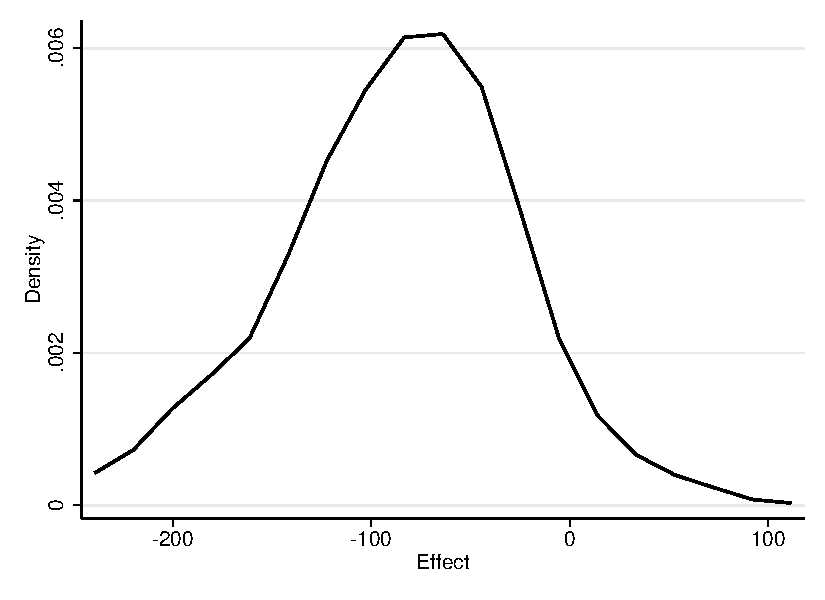
\includegraphics[width=\textwidth]{Figuras/he_dist_fc_admin_disc_pro_2.pdf}
    %\end{subfigure}
    \begin{subfigure}{0.475\textwidth}
        \caption{Effective cost/loan benefit}
        \centering
        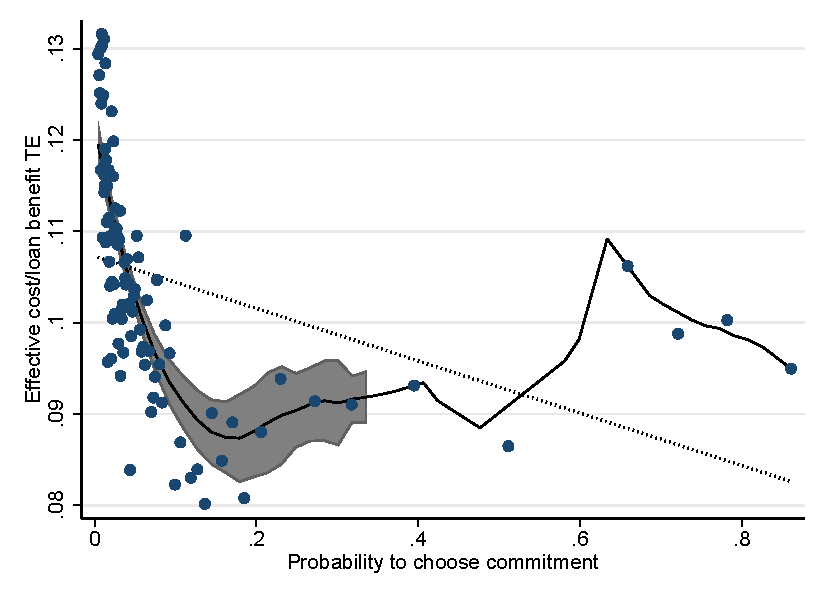
\includegraphics[width=\textwidth]{Figuras/benefit_choice.pdf}
    \end{subfigure}
    \begin{subfigure}{0.475\textwidth}
        \caption{Repayment}
        \centering
        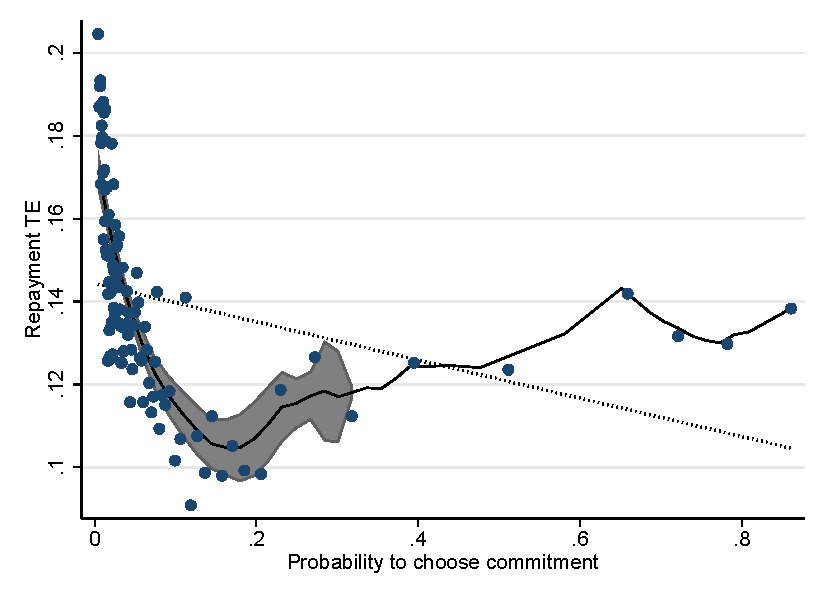
\includegraphics[width=\textwidth]{Figuras/benefit_choice_des.pdf}
    \end{subfigure}
  
    \end{center}
     \scriptsize    Binscatter of propensity to choose commitment vs treatment effect of frequent payments.
          %\footnotesize{ \textit{Do file: }  \texttt{benefit\_choice.do}}
\end{figure}



We estimate demand for commitment with a Gradient Boosted Classification algorithm (accuracy 97\% in-sample and 90\% out-of-sample).


Now we want to identify who are the ones who benefit more from being forced, and those who would demand commitment.


\begin{figure}[H]
    \caption{}
    \label{}
    \begin{center}
    %\begin{subfigure}{0.4\textwidth}
    %    \caption{Financial cost}
    %    \centering
    %    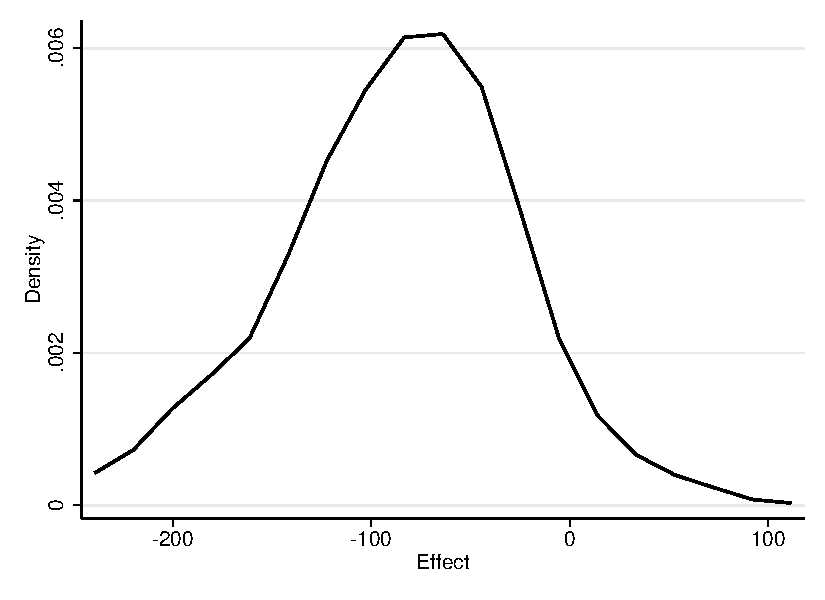
\includegraphics[width=\textwidth]{Figuras/he_dist_fc_admin_disc_pro_2.pdf}
    %\end{subfigure}
    \begin{subfigure}{0.475\textwidth}
        \caption{Determinants of HTE}
        \centering
        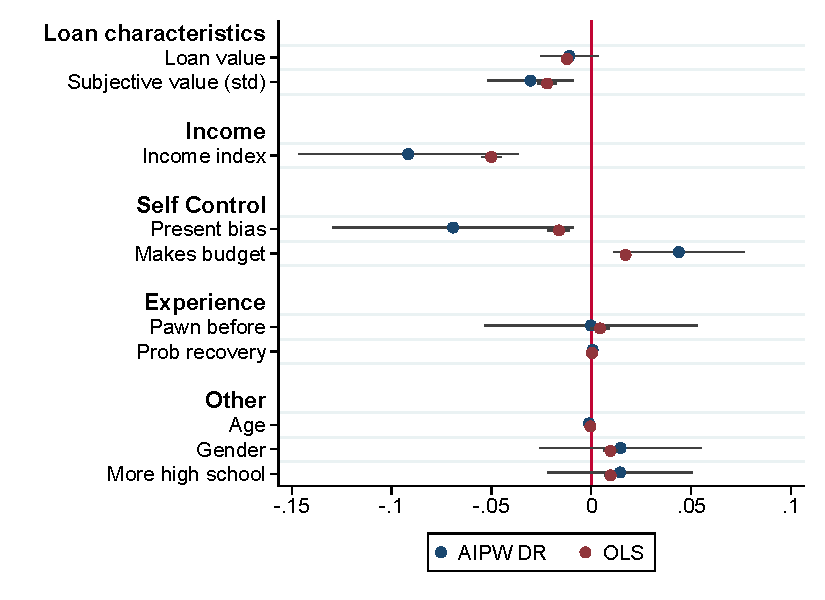
\includegraphics[width=\textwidth]{Figuras/HE/he_int_vertical_eff_cost_loan_pro_2.pdf}
    \end{subfigure}
    \begin{subfigure}{0.475\textwidth}
        \caption{Determinants of PS}
        \centering
        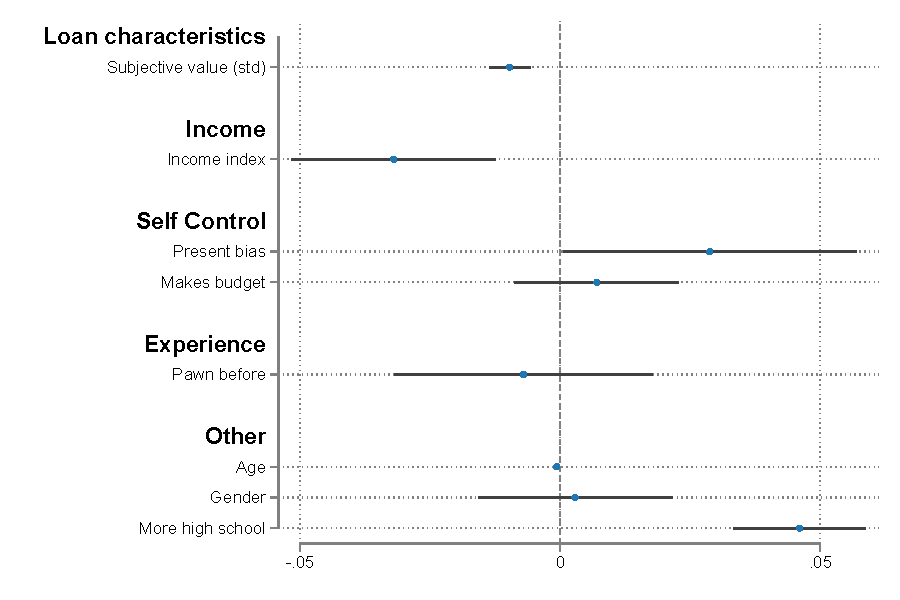
\includegraphics[width=\textwidth]{Figuras/HE/ps_int_vertical_pr_gbc_1.pdf}
    \end{subfigure}
  
    \end{center}
     \scriptsize  (a): This figure estimates bivariate regressions of the estimated client-level heterogeneous treatment effects against the respective covariate from the baseline survey  $\widehat{hte_i} = \alpha + \beta \: X_i + \epsilon_i$. The regressors $X_i$ include (e.g if the family asks for money, if they have savings, if they are overconfident using the definition the text, etc. See this Appendix for a transcription of the survey). \\
     (b) :  
      %\footnotesize{ \textit{Do file: }  \texttt{analyze\_grf\_single\_arm.do}} \texttt{benefit\_choice.do}}
\end{figure}


\subsection{Are the people who benefit most from commitment, the ones who demand it?}

We estimate the following model

We would like to make a distinction of the people that benefit most from being forced. Our conjecture is that this are the naive individuals. 

We assume the following structural model. 


Each individual $i$ is of type  $k\in\{1, 2\}$ with probability $\alpha_{i,k}$. We assume it follows a logit distribution:
\begin{align*}
\label{dist_alpha}
    \alpha_{i,k} = \Pr(\text{Type}_i = k \;|\; \mathbf{W}_{i}) = \frac{e^{\gamma_{k}\mathbf{W}_i}}{\sum_{j=1}^{K} e^{\gamma_{j}\mathbf{W}_i}}
\end{align*}

where $\mathbf{W}_i$ are observable characteristics. This characteristics include choice for commitment, present bias, subjective probability of recovery, etc, which might be indicators of naivete vs sophistication.  

Now, given their type, each individual makes a choice to default or not $c_{i,k} \in \{1,2\}$, based on other set of observable characteristics $\mathbf{X}_i$ (subjective \& objective value of the loan). We will assume there is a continuous latent variable $Y_{i,k,c}$ distributed as
\[Y_{i,k,c} = \beta_{c,k}\mathbf{X}_{i} +\epsilon_{c,k}\]
with\footnote{We can impose other errors, and even impose a covariance structure, for instance if $(\epsilon_{c,k})_{c}\sim\mathcal{N}(0,\Sigma_k)$, we arrive to the Multinomial Probit.} $\epsilon_{c;k}\sim\operatorname{EV}(0,1)$. This latent variable can be thought of as the utility associated with individual $i$, being type $k$, making choice $c$. 



Thus, the density for each individual $i$ being type $k$ is
\[f(c_i,\mathbf{X}_i; \bm\beta_{k}) = \prod_{c=1}^4\left(\frac{e^{\beta_{c,k} \mathbf{X}_i}}{\sum_{j=1}^{4} e^{\beta_{j,k}  \mathbf{X}_i}}\right)^{[c_i=4]}\]

Finally, the generative model is then a mixture model with density given by,
\begin{align*}
    f(c_i ,\mathbf{W}_i, \mathbf{X}_i; \bm{\gamma},\bm{\beta}) &= \sum_{k=1}^K \alpha_k f(c_i,\mathbf{X}_i; \bm\beta_{k}) \\
    &= \sum_{k=1}^K \alpha_k \prod_{c=1}^4\left(\frac{e^{\beta_{c,k} \mathbf{X}_i}}{\sum_{j=1}^{4} e^{\beta_{j,k}  \mathbf{X}_i}}\right)^{[c_i=c]} 
\end{align*}



where $\alpha\sim \operatorname{Categorical}$, and $\gamma_{K} = \beta_{4,k}=0$ for identification purposes. 

Then the (incomplete) log-likelihood function is
\begin{align*}
    \ell(\bm{\gamma}, \bm{\beta}; c, \mathbf{W},  \mathbf{X}) = \sum_{i=1}^n \log\sum_{k=1}^K \alpha_k \prod_{c=1}^4\left(\frac{e^{\beta_{c,k} \mathbf{X}_i}}{\sum_{j=1}^{4} e^{\beta_{j,k}  \mathbf{X}_i}}\right)^{[c_i=c]} 
\end{align*}

, thus we estimate parameters $(\bm{\gamma}, \bm{\beta})$ with an EM algorithm using choice (default)
\& observable characteristics: $(c_i,\mathbf{W}_i,\mathbf{X}_i)$.

The results are the following:

\begin{table}[H]
\caption{FMM}
\label{iv_pf}
\begin{center}
\scriptsize{% Table generated by Excel2LaTeX from sheet 'fmm_types'
\begin{tabular}{lcc}
\cmidrule{1-2}      & Type 1 &  \\
\cmidrule{1-2}      & (1)   &  \\
\cmidrule{1-2}Demand commitment  & -1.73 &  \\
      & (0.76) &  \\
Income index & 3.92  &  \\
      & (3.28) &  \\
Present bias & 0.48  &  \\
      & (0.63) &  \\
Makes budget (almost always) & -1.11 &  \\
      & (0.71) &  \\
Makes budget (always) & 0.068 &  \\
      & (0.54) &  \\
Pawn before & -2.88 &  \\
      & (2.37) &  \\
Prob recovery & -0.011 &  \\
      & (0.014) &  \\
Age   & -0.031 &  \\
      & (0.023) &  \\
Gender & -0.34 &  \\
      & (0.45) &  \\
More than High-School & -1.00 &  \\
      & (0.76) &  \\
Constant & 6.72  &  \\
      & (3.19) &  \\
\cmidrule{1-2}      &       &  \\
      &       &  \\
\midrule
      & \multicolumn{2}{c}{Default} \\
\midrule
      & Type 1 & Type 2 \\
\midrule
\midrule
Loan value (log) & -0.95 & 4.23 \\
      & (0.47) & (1.67) \\
Subjective value & 0.00012 & -0.00080 \\
      & (0.000082) & (0.00035) \\
Constant  & 7.32  & -29.4 \\
      & (3.37) & (11.5) \\
      &       &  \\
\midrule
Observations & 786   & 786 \\
\midrule
Default \% (lower bound) & 0.58  & 0.19 \\
Default \%  & 0.70  & 0.3 \\
Default \% (upper bound) & 0.81  & 0.42 \\
\bottomrule
\bottomrule
\end{tabular}%
}
\end{center}
 \scriptsize

%\textit{Do file: } \texttt{fmm.do}
\end{table}



The class (type) which is positively correlated with demand for commitment might be identified with the \emph{sophisticated} individuals (Type 2). The hypothesis is that this class is the less benefit from being forced, and so (Type 1) individuals are the most benefited from being forced.

\begin{figure}[H]
    \caption{Probability of being Type 1 vs HTE}
    \label{}
    \begin{center}
    \begin{subfigure}{0.475\textwidth}
        \caption{Prior Probability}
        \centering
        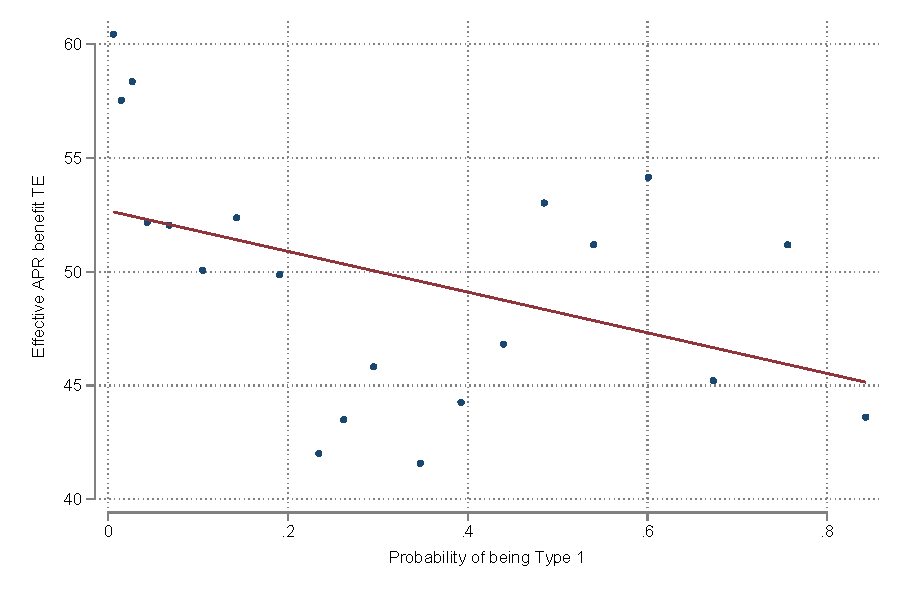
\includegraphics[width=\textwidth]{Figuras/binscatter_tau_classpr.pdf}
    \end{subfigure}
    \begin{subfigure}{0.475\textwidth}
        \caption{Posterior Probability}
        \centering
        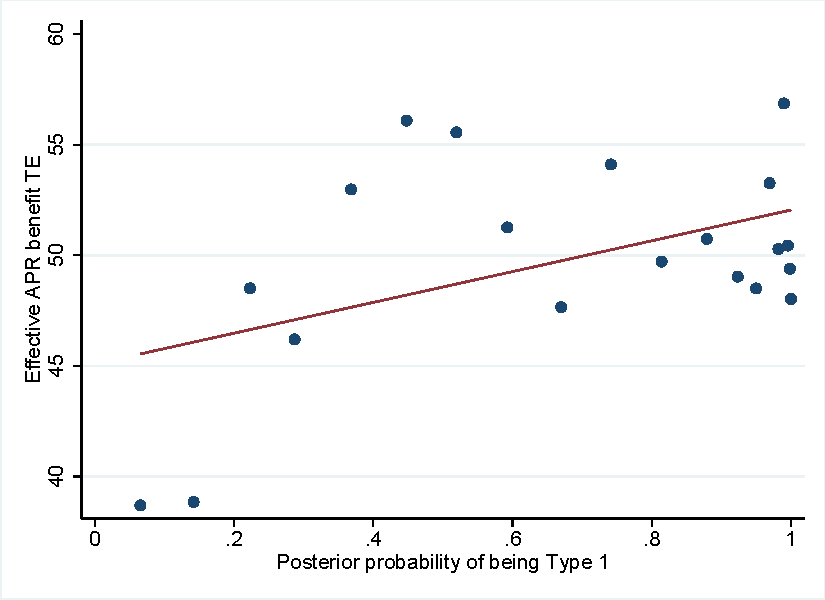
\includegraphics[width=\textwidth]{Figuras/binscatter_tau_classpost.pdf}
    \end{subfigure}
  
    \end{center}
     \scriptsize 
      %\footnotesize{ \textit{Do file: }  \texttt{fmm.do}} 
\end{figure}

A negative relation indicates that being Type 1 has more benefits from being forced.


\begin{figure}[H]
    \caption{Type 1 class vs HTE}
    \label{}
    \begin{center}
    \begin{subfigure}{0.475\textwidth}
        \caption{Prior Probability}
        \centering
        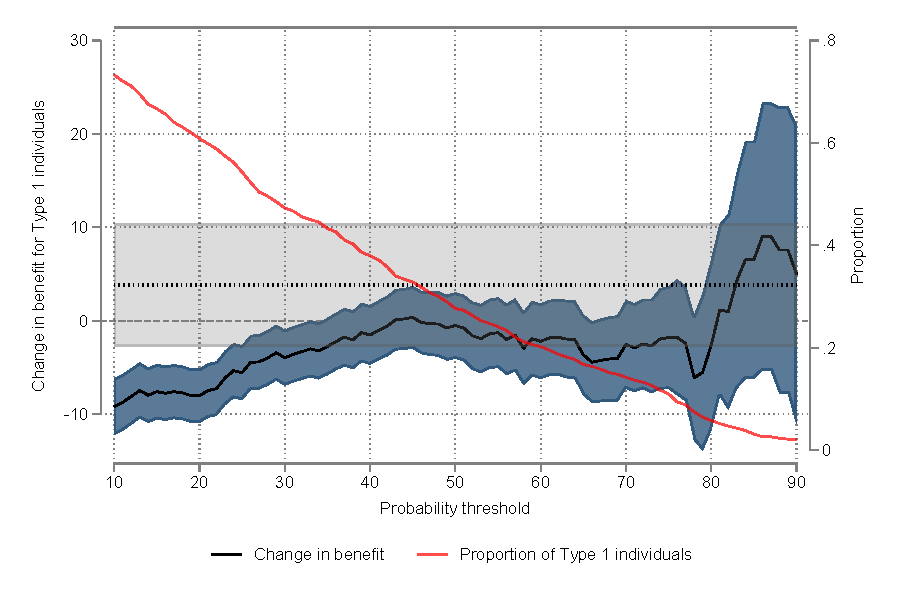
\includegraphics[width=\textwidth]{Figuras/benefit_type1.pdf}
    \end{subfigure}
    \begin{subfigure}{0.475\textwidth}
        \caption{Posterior Probability}
        \centering
        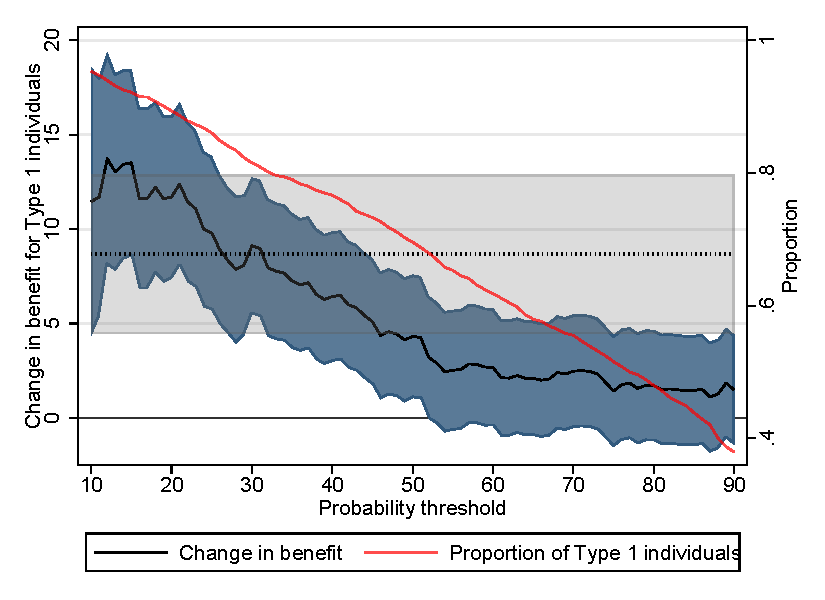
\includegraphics[width=\textwidth]{Figuras/benefit_type1p.pdf}
    \end{subfigure}
  
    \end{center}
     \scriptsize 
      %\footnotesize{ \textit{Do file: }  \texttt{fmm.do}} 
\end{figure}



Moreover we find a strong correlation between the Type 1 individuals and the individuals that ``choose wrong" according to Figure 8 \ref{choose_wrong}.\\

\emph{This exercise is stronger in the sense that when we divide by type, choice is the core divider.} This emphasizes how important choice is as a segregator.


\subsection{Observational Study}

Paternalism  with learning : We generate more learning through forcing than through choice.

It is possible that the wrong people choose and they learn not through choosing, but rather through not choosing (and it did not work). We then partition our sample in the observational study, based on whether you committed the first time, and we want to show that learning happened in the "wrong group" : not choosers.

We want to show that the TE is localized within one of the groups in that endogenous split. 

We then estimate the following two-stage specification.


\begin{equation}
    \mathbbm{1}(\text{Had FP})_{ijt} = \alpha_i + \gamma_t + \beta \mathbbm{1}(\text{FP Avail})_{ijt}  + \epsilon_{ijt}
    \label{eqn:fs}
\end{equation}


\begin{equation}
    \mathbbm{1}(\text{Has FP})_{ijt} = \widehat{\alpha_i }+ \widehat{\gamma_t} + \widehat{\beta }(\widehat{\text{Had FP }})_{ijt}  + \epsilon_{ijt}
    \label{eqn:2s}
\end{equation}



where $i,j,t$ index client, branch, and week respectively. $\mathbbm{1}(\text{Has FP})_{ijt}$ is an indicator for client $i$ pawning in branch $j$ in week $t$ using a FP contract, given that both FP and traditional contracts were available at the branch at the time of pawning, so that there is a choice to be made among these. We instrument $\mathbbm{1}(\text{Had FP previously})_{ijt}$ with the \textit{availability} of the contract in branch $j$  when the client previously went to pawn the immediately prior pawn with respect to $t$, $\mathbbm{1}(\text{FP Avail})_{ijt}$. However, the second stage only uses the subsample of the not choosers. 



\begin{table}[H]
\caption{Outcome in 2S : Choose FP contract}
\label{iv_pf}
\begin{center}
\scriptsize{% Table generated by Excel2LaTeX from sheet 'iv_reg_demand_pf_notchoosing'
\begin{tabular}{lccccc|ccccc}
\toprule
      & \multicolumn{5}{c|}{OLS}              & \multicolumn{5}{c}{FE} \\
\midrule
      & FS    & \multicolumn{2}{c}{IV - 0} & \multicolumn{2}{c|}{Reduced form} & FS    & \multicolumn{2}{c}{IV - 0} & \multicolumn{2}{c}{Reduced form} \\
\midrule
      & (1)   & (2)   & (3)   & (4)   & (5)   & (6)   & (7)   & (8)   & (9)   & (10) \\
\midrule
\midrule
FP available & 0.021 &       &       & 0.011 & 0.00046 & 0.011 &       &       & 0.0038 & 0.0064 \\
      & (0.00066) &       &       & (0.0014) & (0.0013) & (0.00090) &       &       & (0.0018) & (0.0018) \\
Had FP in the past &       & 0.50  & 0.022 &       &       &       & 0.35  & 0.60  &       &  \\
      &       & (0.065) & (0.064) &       &       &       & (0.17) & (0.17) &       &  \\
Residual &       & -0.019 &       &       &       &       & -0.55 &       &       &  \\
      &       & (0.064) &       &       &       &       & (0.17) &       &       &  \\
\midrule
Observations & $>$100000 & $>$100000 & $>$100000 & $>$100000 & \multicolumn{1}{c}{$>$100000} & 70\%  & 70\%  & 70\%  & 70\%  & 70\% \\
R-sq  & 0.013 & 0.089 & 0.021 & 0.020 & 0.021 & 0.581 & 0.564 & 0.492 & 0.559 & 0.492 \\
DepVarMean & 0.013 & 0.045 & 0.039 & 0.045 & 0.039 & 0.012 & 0.038 & 0.029 & 0.038 & 0.029 \\
\midrule
Conditional not choose &       &       & \checkmark &       & \checkmark &       &       & \checkmark &       & \checkmark \\
Calendar week FE & \checkmark & \checkmark & \checkmark & \checkmark & \checkmark & \checkmark & \checkmark & \checkmark & \checkmark & \checkmark \\
Branch FE & \checkmark & \checkmark & \checkmark & \checkmark & \checkmark & \checkmark & \checkmark & \checkmark & \checkmark & \checkmark \\
Client FE &       &       &       &       &       & \checkmark & \checkmark & \checkmark & \checkmark & \checkmark \\
\midrule
\midrule
      &       &       &       &       & \multicolumn{1}{c}{} &       &       &       &       &  \\
\midrule
      & \multicolumn{5}{c|}{OLS}              & \multicolumn{5}{c}{FE} \\
\midrule
      & FS    & \multicolumn{2}{c}{IV - 1} & \multicolumn{2}{c|}{Reduced form} & FS    & \multicolumn{2}{c}{IV - 1} & \multicolumn{2}{c}{Reduced form} \\
\midrule
      & (11)  & (12)  & (13)  & (14)  & (15)  & (16)  & (17)  & (18)  & (19)  & (20) \\
\midrule
\midrule
FP available & 0.020 &       &       & 0.0088 & -0.000083 & 0.0099 &       &       & 0.0034 & 0.0063 \\
      & (0.00067) &       &       & (0.0015) & (0.0014) & (0.00096) &       &       & (0.0020) & (0.0020) \\
Had FP in the past &       & 0.43  & -0.0041 &       &       &       & 0.35  & 0.64  &       &  \\
      &       & (0.071) & (0.070) &       &       &       & (0.20) & (0.20) &       &  \\
Residual &       & 0.0069 &       &       &       &       & -0.57 &       &       &  \\
      &       & (0.070) &       &       &       &       & (0.20) &       &       &  \\
\midrule
Observations & $\sim$100000 & $\sim$100000 & $\sim$100000 & $\sim$100000 & $\sim$100000 & 70\%  & 70\%  & 70\%  & 70\%  & 70\% \\
R-sq  & 0.013 & 0.080 & 0.024 & 0.022 & 0.024 & 0.577 & 0.545 & 0.483 & 0.539 & 0.483 \\
DepVarMean & 0.013 & 0.043 & 0.037 & 0.043 & 0.037 & 0.010 & 0.035 & 0.027 & 0.035 & 0.027 \\
\midrule
Conditional not choose &       &       & \checkmark &       & \checkmark &       &       & \checkmark &       & \checkmark \\
Calendar week FE & \checkmark & \checkmark & \checkmark & \checkmark & \checkmark & \checkmark & \checkmark & \checkmark & \checkmark & \checkmark \\
Branch FE & \checkmark & \checkmark & \checkmark & \checkmark & \checkmark & \checkmark & \checkmark & \checkmark & \checkmark & \checkmark \\
Client FE &       &       &       &       &       & \checkmark & \checkmark & \checkmark & \checkmark & \checkmark \\
\bottomrule
\bottomrule
\end{tabular}%
}
\end{center}
 \scriptsize

%\textit{Do file: } \texttt{iv\_reg\_demand\_pf\_notchoosing.do}
\end{table}

Thus the learning mechanism is due to the not choosers having failed. 





\begin{table}[H]
\caption{Outcome in 2S : Default}
\label{iv_def}
\begin{center}
\scriptsize{% Table generated by Excel2LaTeX from sheet 'iv_reg_def_notchoosing'
\begin{tabular}{lccccc|ccccc}
\toprule
      & \multicolumn{5}{c|}{OLS}              & \multicolumn{5}{c}{FE} \\
\midrule
      & FS    & \multicolumn{2}{c}{IV - 0} & \multicolumn{2}{c|}{Reduced form} & FS    & \multicolumn{2}{c}{IV - 0} & \multicolumn{2}{c}{Reduced form} \\
\midrule
      & (1)   & (2)   & (3)   & (4)   & (5)   & (6)   & (7)   & (8)   & (9)   & (10) \\
\midrule
\midrule
FP available & 0.021 &       &       & -0.0087 & -0.0015 & 0.011 &       &       & -0.00037 & -0.0024 \\
      & (0.00065) &       &       & (0.0031) & (0.0031) & (0.00088) &       &       & (0.0045) & (0.0046) \\
Had FP in the past &       & -0.42 & -0.073 &       &       &       & -0.035 & -0.23 &       &  \\
      &       & (0.15) & (0.15) &       &       &       & (0.43) & (0.43) &       &  \\
Residual &       & 0.066 &       &       &       &       & 0.16  &       &       &  \\
      &       & (0.15) &       &       &       &       & (0.43) &       &       &  \\
\midrule
Observations & $>$100000 & $>$100000 & $>$100000 & $>$100000 & \multicolumn{1}{c}{$>$100000} & 70\%  & 70\%  & 70\%  & 70\%  & 70\% \\
R-sq  & 0.012 & 0.013 & 0.005 & 0.005 & 0.005 & 0.585 & 0.516 & 0.510 & 0.515 & 0.510 \\
DepVarMean & 0.013 & 0.73  & 0.74  & 0.73  & 0.74  & 0.011 & 0.71  & 0.72  & 0.71  & 0.72 \\
\midrule
Conditional not choose &       &       & \checkmark &       & \checkmark &       &       & \checkmark &       & \checkmark \\
Calendar week FE & \checkmark & \checkmark & \checkmark & \checkmark & \checkmark & \checkmark & \checkmark & \checkmark & \checkmark & \checkmark \\
Branch FE & \checkmark & \checkmark & \checkmark & \checkmark & \checkmark & \checkmark & \checkmark & \checkmark & \checkmark & \checkmark \\
Client FE &       &       &       &       &       & \checkmark & \checkmark & \checkmark & \checkmark & \checkmark \\
\midrule
\midrule
      &       &       &       &       & \multicolumn{1}{c}{} &       &       &       &       &  \\
\midrule
      & \multicolumn{5}{c|}{OLS}              & \multicolumn{5}{c}{FE} \\
\midrule
      & FS    & \multicolumn{2}{c}{IV - 1} & \multicolumn{2}{c|}{Reduced form} & FS    & \multicolumn{2}{c}{IV - 1} & \multicolumn{2}{c}{Reduced form} \\
\midrule
      & (11)  & (12)  & (13)  & (14)  & (15)  & (16)  & (17)  & (18)  & (19)  & (20) \\
\midrule
\midrule
FP available & 0.020 &       &       & -0.0094 & -0.0027 & 0.0097 &       &       & -0.0022 & -0.0041 \\
      & (0.00067) &       &       & (0.0032) & (0.0032) & (0.00095) &       &       & (0.0049) & (0.0049) \\
Had FP in the past &       & -0.47 & -0.14 &       &       &       & -0.22 & -0.42 &       &  \\
      &       & (0.16) & (0.16) &       &       &       & (0.51) & (0.51) &       &  \\
Residual &       & 0.13  &       &       &       &       & 0.37  &       &       &  \\
      &       & (0.16) &       &       &       &       & (0.51) &       &       &  \\
\midrule
Observations & $\sim$100000 & $\sim$100000 & $\sim$100000 & $\sim$100000 & $\sim$100000 & 70\%  & 70\%  & 70\%  & 70\%  & 70\% \\
R-sq  & 0.013 & 0.012 & 0.005 & 0.005 & 0.005 & 0.583 & 0.528 & 0.524 & 0.528 & 0.524 \\
DepVarMean & 0.012 & 0.74  & 0.75  & 0.74  & 0.75  & 0.0099 & 0.73  & 0.73  & 0.73  & 0.73 \\
\midrule
Conditional not choose &       &       & \checkmark &       & \checkmark &       &       & \checkmark &       & \checkmark \\
Calendar week FE & \checkmark & \checkmark & \checkmark & \checkmark & \checkmark & \checkmark & \checkmark & \checkmark & \checkmark & \checkmark \\
Branch FE & \checkmark & \checkmark & \checkmark & \checkmark & \checkmark & \checkmark & \checkmark & \checkmark & \checkmark & \checkmark \\
Client FE &       &       &       &       &       & \checkmark & \checkmark & \checkmark & \checkmark & \checkmark \\
\bottomrule
\bottomrule
\end{tabular}%
}
\end{center}
 \scriptsize

%\textit{Do file: } \texttt{iv\_reg\_demand\_pf\_notchoosing.do}
\end{table}

\begin{table}[H]
\caption{Outcome in 2S : Default}
\label{iv_def_decomp}
\begin{center}
\scriptsize{% Table generated by Excel2LaTeX from sheet 'iv_reg_def_nc_nr'
\begin{tabular}{lcccccccc}
\toprule
\multicolumn{9}{c}{IV-0} \\
\midrule
      & Refrendum & \multicolumn{7}{c}{Default} \\
\midrule
      & (1)   & (2)   & (3)   & (4)   & (5)   & (6)   & (7)   & (8) \\
\midrule
\midrule
Had FP in the past &       &       & -0.064 & -1.72 & -0.27 & -1.90 & -0.15 & -0.40 \\
      &       &       & (0.47) & (0.73) & (0.47) & (0.73) & (0.71) & (0.71) \\
FP    & -0.64 & -0.77 &       &       &       &       &       &  \\
      & (0.043) & (0.036) &       &       &       &       &       &  \\
Residual & 0.0016 & 0.046 & 0.19  &       &       &       &       &  \\
      & (0.043) & (0.036) & (0.47) &       &       &       &       &  \\
Had FP in the past\#Not refrendum &       &       &       &       &       &       & -1.02 & -0.87 \\
      &       &       &       &       &       &       & (0.78) & (0.78) \\
Not refrendum &       &       &       &       &       &       & -0.26 & -0.26 \\
      &       &       &       &       &       &       & (0.0088) & (0.0088) \\
\midrule
Observations & 773596 & 773596 & 77215 & 34802 & 76106 & 34104 & 77215 & 76106 \\
R-sq  & 0.447 & 0.463 & 0.554 & 0.644 & 0.550 & 0.639 & 0.595 & 0.590 \\
DepVarMean & 0.51  & 0.74  & 0.73  & 0.65  & 0.73  & 0.66  & 0.73  & 0.73 \\
\midrule
Conditional not choose &       &       &       &       & \checkmark & \checkmark &       & \checkmark \\
Conditional on not refrendum &       &       &       & \checkmark &       & \checkmark & -     & - \\
Calendar week FE & \checkmark & \checkmark & \checkmark & \checkmark & \checkmark & \checkmark & \checkmark & \checkmark \\
Branch FE & \checkmark & \checkmark & \checkmark & \checkmark & \checkmark & \checkmark & \checkmark & \checkmark \\
Client FE & \checkmark & \checkmark & \checkmark & \checkmark & \checkmark & \checkmark & \checkmark & \checkmark \\
\midrule
\midrule
      &       &       &       &       &       &       &       &  \\
\midrule
\multicolumn{9}{c}{IV-1} \\
\midrule
      &       &       & \multicolumn{6}{c}{Default} \\
\midrule
      &       &       & (9)   & (10)  & (11)  & (12)  & (13)  & (14) \\
\midrule
\midrule
Had FP in the past &       &       & -0.23 & -1.54 & -0.44 & -1.69 & -0.42 & -0.68 \\
      &       &       & (0.54) & (0.83) & (0.54) & (0.84) & (0.78) & (0.79) \\
Residual &       &       & 0.37  &       &       &       &       &  \\
      &       &       & (0.54) &       &       &       &       &  \\
Had FP in the past\#Not refrendum &       &       &       &       &       &       & -0.82 & -0.67 \\
      &       &       &       &       &       &       & (0.80) & (0.80) \\
Not refrendum &       &       &       &       &       &       & -0.25 & -0.25 \\
      &       &       &       &       &       &       & (0.0094) & (0.0094) \\
\midrule
Observations &       &       & 64383 & 29329 & 63523 & 28838 & 64383 & 63523 \\
R-sq  &       &       & 0.571 & 0.655 & 0.568 & 0.650 & 0.607 & 0.604 \\
DepVarMean &       &       & 0.74  & 0.67  & 0.75  & 0.68  & 0.74  & 0.75 \\
\midrule
Conditional not choose &       &       &       &       & \checkmark & \checkmark &       & \checkmark \\
Conditional on not refrendum &       &       &       & \checkmark &       & \checkmark & -     & - \\
Calendar week FE &       &       & \checkmark & \checkmark & \checkmark & \checkmark & \checkmark & \checkmark \\
Branch FE &       &       & \checkmark & \checkmark & \checkmark & \checkmark & \checkmark & \checkmark \\
Client FE &       &       & \checkmark & \checkmark & \checkmark & \checkmark & \checkmark & \checkmark \\
\bottomrule
\bottomrule
\end{tabular}%
}
\end{center}
 \scriptsize

%\textit{Do file: } \texttt{iv\_reg\_demand\_pf\_notchoosing.do}
\end{table}

\section{LATE}

\begin{table}[H]
\caption{}
\label{tot_tut}
\begin{center}
\scriptsize{% Table generated by Excel2LaTeX from sheet 'tot_tut_iv'
\begin{tabular}{lcccccc|cc}
\toprule
      & \multicolumn{6}{c|}{Effective cost/loan benefit} & \multicolumn{2}{c}{CATE - CF} \\
\midrule
      & (1)   & (2)   & (3)   & (4)   & (5)   & (6)   & (7)   & (8) \\
\midrule
\midrule
TOT   & 0.051 & 0.072 & 0.074 &       &       &       &       &  \\
      & (0.13) & (0.11) & (0.085) &       &       &       &       &  \\
TUT   &       &       &       & 0.11  & 0.11  & 0.11  &       &  \\
      &       &       &       & (0.020) & (0.020) & (0.015) &       &  \\
Choose commitment &       &       &       &       &       &       & -0.0064 & -0.010 \\
      &       &       &       &       &       &       & (0.0036) & (0.0038) \\
\midrule
Observations & 1863  & 1863  & 1863  & 1891  & 1891  & 1891  & 1018  & 1018 \\
R-sq  & 0.011 & 0.044 & 0.050 & 0.053 & 0.069 & 0.073 & 0.003 & 0.114 \\
DepVarMean & \multicolumn{6}{c|}{0.11}                     & 0.10  & 0.10 \\
Randomization inference p-value &       &       &       &       &       &       & 0.088 & 0.0050 \\
Admin controls &       & \checkmark & \checkmark &       & \checkmark & \checkmark &       & \checkmark \\
Survey Controls &       &       & \checkmark &       &       & \checkmark &       &  \\
\bottomrule
\bottomrule
\end{tabular}%
}
\end{center}
 \scriptsize
%\textit{Do file: } \texttt{tot\_tut.do}
\end{table}


\begin{figure}[H]
     \caption{TOT-TUT Histogram}
    \label{}
    \begin{center}
    \begin{subfigure}{0.75\textwidth}
        \centering
        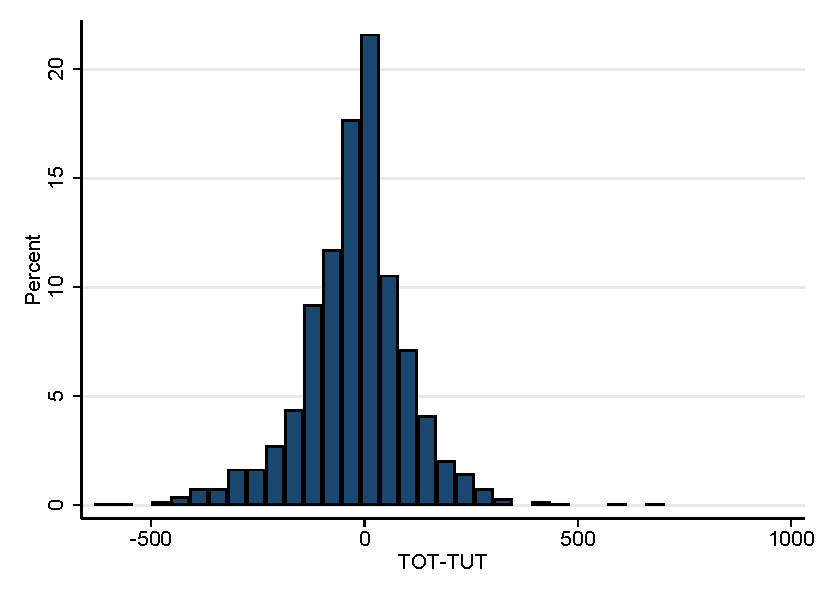
\includegraphics[width=\textwidth]{Figuras/dif_tot_tut.pdf}
    \end{subfigure}
    \end{center}
    \scriptsize
        Histogram for the difference of the conditional (heterogeneous) TOT-TUT
          %\footnotesize{ \textit{Do file: }  \texttt{tot\_tut\_insforest.do}}
\end{figure}


\begin{figure}[H]
     \caption{TOT-TUT CDF}
    \label{ExplanatoryMaterial}
    \begin{center}
    \begin{subfigure}{0.75\textwidth}
        \centering
        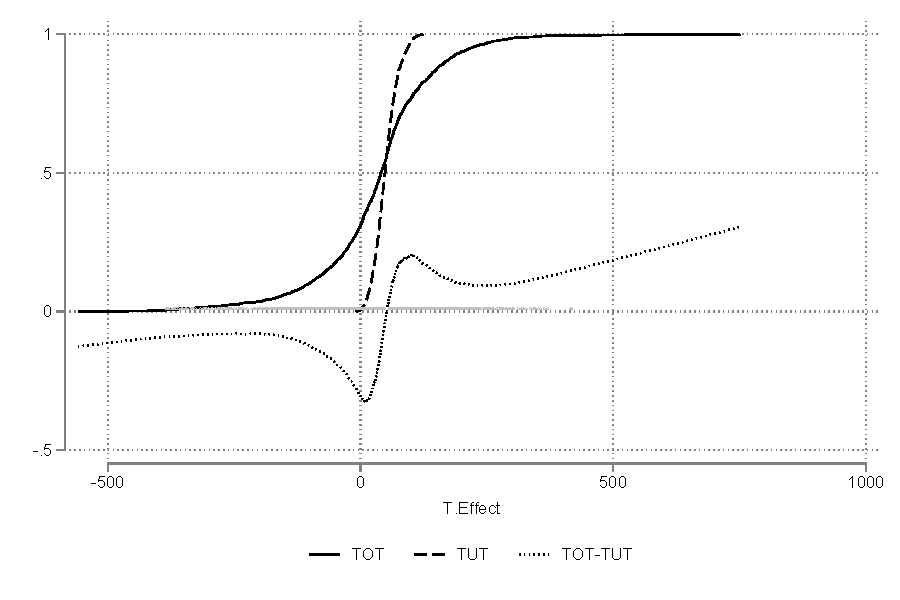
\includegraphics[width=\textwidth]{Figuras/cdf_tot_tut.pdf}
    \end{subfigure}
    \end{center}
    \scriptsize
        ECDF of the conditional (heterogeneous) TOT \& TUT, alogn with the difference and a test for the difference in means (which is significant).
          %\footnotesize{ \textit{Do file: }  \texttt{tot\_tut\_insforest.do}}
\end{figure}


\newpage
\section{Appendix : Mixture Model}
Mixing distributions and mixture models are able to approximate the density function of any unknown distribution to arbitrary degrees of accuracy, provided that the mixing or mixture distribution  is  sufficiently  complex \cite{nguyen}. In fact, \cite{mcfadden} demonstrated that any random utility model can be approximated to any degree of accuracy by a mixed logit with the appropriate specification of variables and mixing distribution. We follow the approach by \cite{TRAIN200840}.\\



\subsection{Estimation}

The EM algorithm following \cite{em,em_seq} but most importantly \cite{TRAIN200840}, is in our setting :

\begin{algorithm}[H]
\SetKwInOut{Input}{input}\SetKwInOut{Output}{output}

\caption{EM}\label{EM}
\small{
\Input{$(c_i, \mathbf{W}_i,  \mathbf{X}_i)$}
\Output{$\hat{\bm\gamma}, \hat{\bm{\beta}}, \widetilde{\alpha_{i,k}}, \widetilde{\alpha_{k}}$}
\BlankLine
Initialize $\gamma_{k}^{(0)}, \beta_k^{(0)}$

Update the predicted probability (weight) for individual $i$, type $k$: \;
$\widehat{\alpha_{i,k}^{(0)}} = \frac{e^{\gamma_{k}^{(0)}\mathbf{W}_i}}{\sum_{j=1}^{K} e^{\gamma_{j}^{(0)}\mathbf{W}_i}} $
% $\alpha_{i}^{(0)}\sim \operatorname{Categorical}$, following (\ref{dist_alpha})

Update the shares of types:\;
$\widehat{\alpha_k^{(0)}} = \frac{\sum_{i=1}^n\widehat{\alpha_{i,k}^{(0)}}}{\sum_{k=1}^{K}\sum_{i=1}^n\widehat{\alpha_{i,k}^{(0)}}}$\;

\textbf{E-step :}

Compute predicted posterior probability  for the $k$ type: \;
$\widetilde{\alpha_{i,k}^{(0)}} = \frac{\widehat{\alpha_k^{(0)}}f(c_i,\mathbf{X}_i; \bm\beta_{k}^{(0)})}{\sum_{k=1}^K\widehat{\alpha_k^{(0)}}f(c_i,\mathbf{X}_i; \bm\beta_{k}^{(0)})}$\;


\While{$||(\bm\gamma^{(t)},\bm\beta^{(t)})-(\bm\gamma^{(t-1)},\bm\beta^{(t-1)})||>\operatorname{tol}$}{


\textbf{M-step :}


$\bm\beta_{k}^{(t+1)}  = \operatorname{argmax}_{\bm\beta_{k}} \sum_{i=1}^n \widetilde{\alpha_{i,k}^{(t)}} \log \prod_{c=1}^4\left(\frac{e^{\beta_{c,k} \mathbf{X}_i}}{\sum_{j=1}^{4} e^{\beta_{j,k}  \mathbf{X}_i}}\right)^{[c_i=c]} $\;
\scriptsize{(Run a multinomial-logit model with weighted observations, with weights given by the conditional probabilities of type membership)}\;
\small

$\bm\gamma_{k}^{(t+1)} = \operatorname{argmax}_{\bm\gamma_{k}} \sum_{i=1}^n\sum_{k=1}^K \widetilde{\alpha_{i,k}^{(t)}} \log \left(\frac{e^{\gamma_{k}\mathbf{W}_i}}{\sum_{j=1}^{K} e^{\gamma_{j}\mathbf{W}_i}}\right) $\;

\scriptsize{(Grouped-data log likelihood, where we have used a multinomial-logit specification)}\;

\small

Update the predicted probability (weight) for individual $i$, type $k$: \;
$\widehat{\alpha_{i,k}^{(t+1)}} = \frac{e^{\gamma_{k}^{(t+1)}\mathbf{W}_i}}{\sum_{j=1}^{K} e^{\gamma_{j}^{(t+1)}\mathbf{W}_i}} $
% $\alpha_{i}^{(0)}\sim \operatorname{Categorical}$, following (\ref{dist_alpha})

Update the shares of types:\;
$\widehat{\alpha_k^{(t+1)}} = \frac{\sum_{i=1}^n\widehat{\alpha_{i,k}^{(t+1)}}}{\sum_{k=1}^{K}\sum_{i=1}^n\widehat{\alpha_{i,k}^{(t+1)}}}$\;


\textbf{E-step :}

Compute predicted posterior probability  for the $k$ type: \;
$\widetilde{\alpha_{i,k}^{(t+1)}} = \frac{\widehat{\alpha_k^{(t+1)}}f(c_i,\mathbf{X}_i; \bm\beta_{k}^{(t+1)})}{\sum_{k=1}^K\widehat{\alpha_k^{(t+1)}}f(c_i,\mathbf{X}_i; \bm\beta_{k}^{(t+1)})}$\;


}
Update the posterior shares of types:\;
$\widetilde{\alpha_k^{(t+1)}} = \frac{\sum_{i=1}^n\widetilde{\alpha_{i,k}^{(t+1)}}}{\sum_{k=1}^{K}\sum_{i=1}^n\widetilde{\alpha_{i,k}^{(t+1)}}}$\;
}
\end{algorithm}


\subsection{Extensions}

A stochastic version\footnote{See \cite{nielsen}.} of the estimation above consists, at iteration $t$, in replacing the probability of the unknown types $k$ by a sequence sampled from a Categorical distribution
\[\widehat{\alpha_{i}^{(t)}}\sim \operatorname{Categorical}\left(\frac{\widehat{\alpha_k^{(t+1)}}f(c_i,\mathbf{X}_i; \bm\beta_{k}^{(t+1)})}{\sum_{k=1}^K\widehat{\alpha_k^{(t+1)}}f(c_i,\mathbf{X}_i; \bm\beta_{k}^{(t+1)})}\right)\] 
We call this the \textbf{SE-step}. We can then use these sampled labels for updating the estimation in the \textbf{M-step} by maximizing the \emph{complete} maximum likelihood. 
 
 
\subsubsection{Degrees of naivete}
We can model degrees of naivete assuming every individual $i$ has a (continuous) propensity of being of each type. We model this by making the predicted probability of each individual follow a Dirichlet regression $\alpha_{i} \sim \operatorname{DirichletReg}$.


\subsection{Identifiability}
\cite{grun} analyze the identifiability of a general class of finite mixtures of multinomial logits.



\newpage
\clearpage
\bibliographystyle{authordate1}
%\bibliographystyle{amsalpha}
%\bibliographystyle{AER}

\bibliography{References_aux.bib}


\end{document}
